%! TeX program = lualatex
\documentclass[a4paper,11pt]{article} 
% packages
\usepackage{fontspec}
\setmainfont{EB Garamond}
% for tironian et fallback
% % \directlua{luaotfload.add_fallback
% % ("emojifallback",
% %      {"Noto Serif:mode=harf"}
% % )}
% % \setmainfont{EB Garamond}[RawFeature={fallback=emojifallback}]

\setmonofont[Scale=MatchLowercase]{Deja Vu Sans Mono}
\usepackage[a4paper,left=2cm,right=2cm,top=\dimexpr15mm+1.5\baselineskip,bottom=2cm]{geometry}
\setlength{\parindent}{0pt}

\usepackage{fancyhdr}       % Headers and footers 
\fancyhead[R]{\normalfont \leftmark}
\fancyhead[L]{}
\pagestyle{fancy}

\usepackage{multicol}       
\usepackage{microtype}      % Slightly tweak font spacing for aesthetics
\usepackage[english]{babel} % Language hyphenation and typographical rules
\usepackage[final, colorlinks = true, urlcolor = blue, linkcolor = black]{hyperref} 
% \urlstyle{tt}
\usepackage{changepage}     % adjust margins on the fly

\usepackage{minted}
\usemintedstyle{algol_nu}
\usepackage{xcolor}

\usepackage{pgfplots}
\pgfplotsset{width=\textwidth,compat=1.9}

\usepackage{caption}
\newenvironment{code}{\captionsetup{type=listing}}{}

\usepackage[yyyymmdd]{datetime}
\renewcommand{\dateseparator}{-}

\usepackage{titlesec}

\begin{document}
\begin{titlepage}
    \begin{center}
        \hrule
        \vspace*{0.6cm}
        \huge \textbf{CT3536}
        \vspace*{0.6cm}
        \hrule
        \LARGE
       \vspace{0.5cm}
        GAMES PROGRAMMING
       \vspace{0.5cm}
       \hrule
            
       \vfill
       
\includegraphics[width=0.8\textwidth]{images/unity-logo.png}
        \vfill

        \Large
       \vspace{0.5cm}
       \hrule
       \vspace{0.5cm}
       \textbf{Andreas Ó hAoḋa}
       % \vspace{0.5cm}
       % \hrule
       % \vspace{0.5cm}
            
       \normalsize
       University of Galway

       \today

       \vspace{0.5cm}
       \hrule
    \end{center}
\end{titlepage}

\pagenumbering{roman}
\newpage
\tableofcontents
\newpage
\setcounter{page}{1}
\pagenumbering{arabic}

\section{Introduction}
\subsection{Lecturer Contact Information}
\begin{itemize}
    \item   Dr. Sam Redfern (\href{mailto://sam.redfern@nuigalway.ie}{\texttt{sam.redfern@nuigalway.ie}})
    \item   Discord server: \url{https://discord.gg/nqD5JN95WT}
\end{itemize}

\subsection{Assessment}
There will be 1-3 person projects which will begin from approximately Week 5, which will be worth 30\% of the course marks.
10\% of the overall mark will be from the six graded lab assignments, and the remaining 60\% will be from the final exam.
\\\\ 
The game project will have a demo in the final week, and will be submitted as a document containing images, discussions, 
code, etc. 
Marks are awarded for:
\begin{itemize}
    \item   Overall complexity.
    \item   Code architecture \& neatness. 
    \item   Game design/elegance \& UX. 
    \item   Discussion.
    \item   Graphics (if self-created).
    \item   Audio (if self-control).
    \item   Group size will also be taken into account.
\end{itemize}

You should start to consider your ideas by Week 5. 
Discuss the idea with Dr. Redfern \& the lab tutors as they can advise on scope \& difficulty.
Simple 3D games are no harder to make than 2D games. 
``Snake'' games are not allowd!'


\subsection{Game Engines}
\textbf{Game Engines} provide a powerful set of integrated sub-systems geared towards making games (and other high-performance
\emph{realtime} media) including:
\begin{itemize}
    \item   Graphics Rendering (3D, 2D, terrain).
    \item   Physics.
    \item   Networking.
    \item   Special Effects. 
    \item   3D Audio.
    \item   User Input.
\end{itemize}

\subsection{Unity3D Game Engine}
The Unity3D game engine is a closed-source games engine that is well designed \& elegant to use ``2\textsuperscript{nd}
generation'' game engine. 
It has excellent GUI/HUD editing \& animation system, and is powerful \& very popular. 
It has a hugely successful Asset Store. 
Its core language is C\#, which is very similar to Java. 
Unity3D deploys to iOS, Android, Web (HTML5/WebGL), Windows, Mac OSX, Linux, Switch, \& more.
\begin{figure}[H]
    \centering
    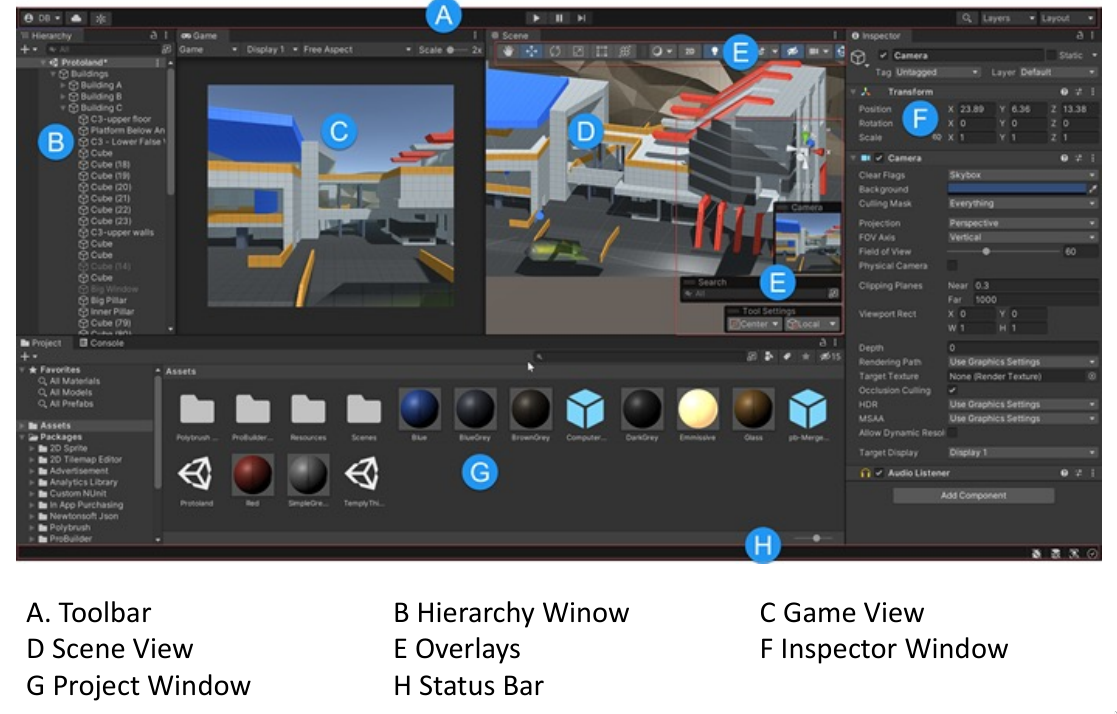
\includegraphics[width=0.9\textwidth]{./images/unity_ide.png}
    \caption{The Unity IDE}
\end{figure}

The \textbf{Project Window} displays your library of assets that are available to use in your project. 
When you import assets into your project, they appear here.
\begin{figure}[H]
    \centering
    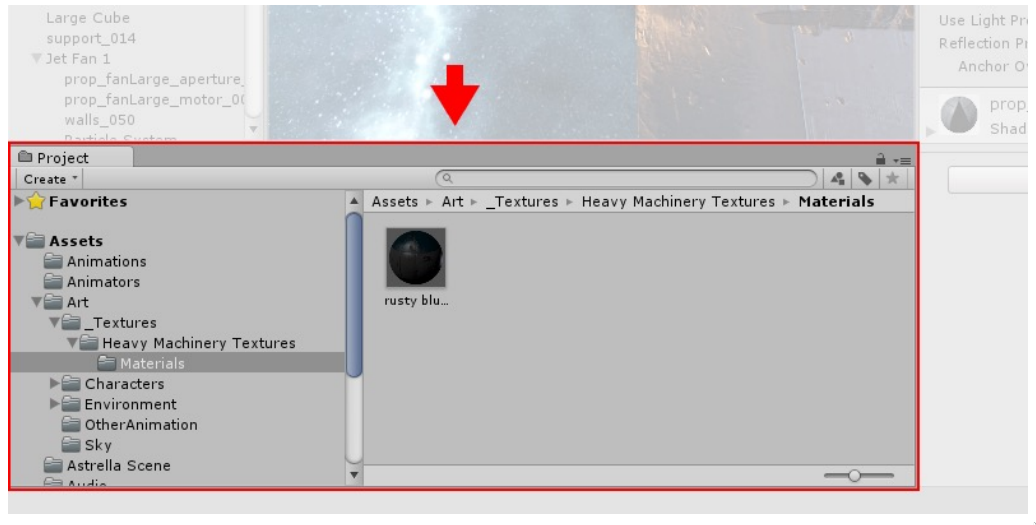
\includegraphics[width=0.9\textwidth]{./images/project_window.png}
    \caption{The Project Window (Assets)}
\end{figure}

The \textbf{Scene View} allows you to visually navigate \& edit your scene without running your game. 
The scene view can be a 3D or 2D perspective.
\begin{figure}[H]
    \centering
    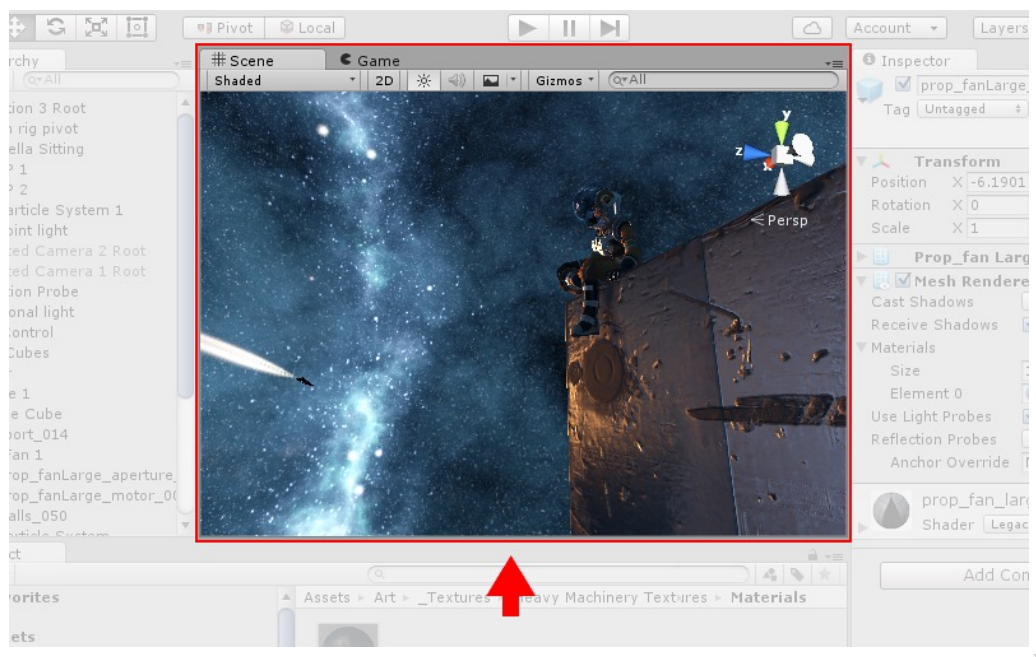
\includegraphics[width=0.9\textwidth]{./images/scene_view.png}
    \caption{The Scene View}
\end{figure}

The \textbf{Hierarchy Window} is a hierarchical nested text representation of every ``\textbf{game object}'' in the scene.
\begin{figure}[H]
    \centering
    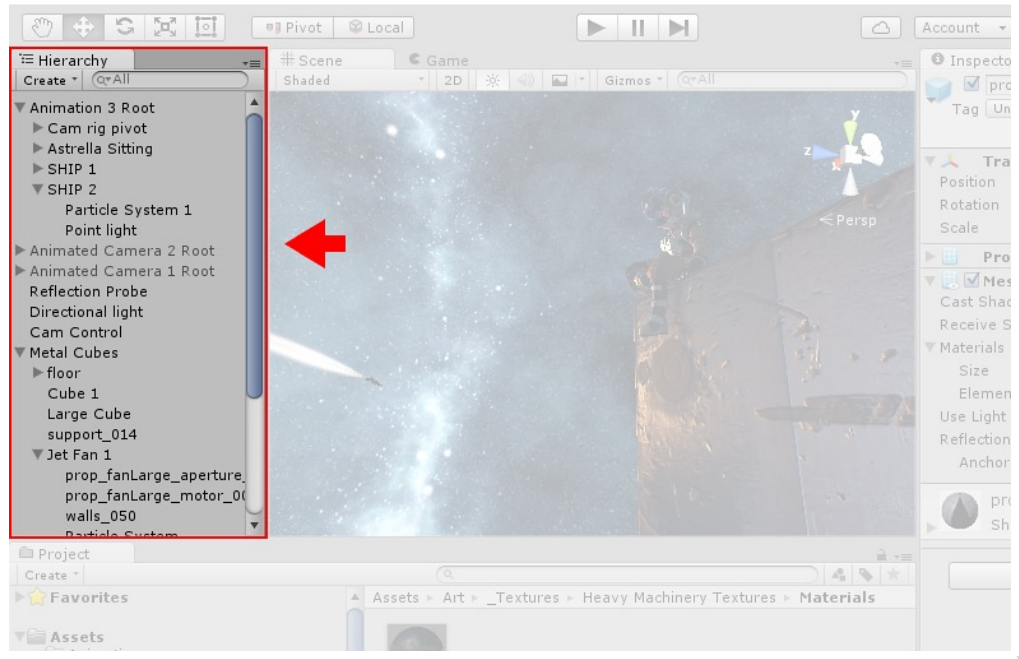
\includegraphics[width=0.9\textwidth]{./images/hierarchy_window.png}
    \caption{The Hierarchy (Scene Graph) Window}
\end{figure}

The \textbf{Inspector Window} allows you to view \& edit all the properties of the currently selected game object.
\begin{figure}[H]
    \centering
    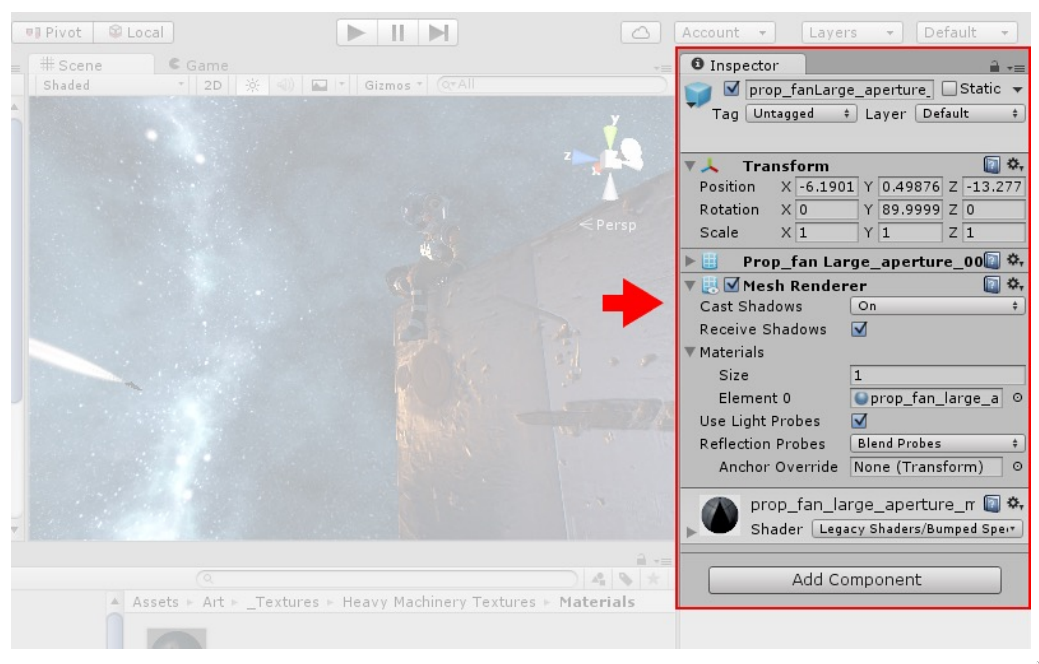
\includegraphics[width=0.9\textwidth]{./images/inspector_window.png}
    \caption{The Inspector Window}
\end{figure}

The \textbf{toolbar} provides access to the most essential working features. 
On the left it contains the basic tools for manipulating the scene view \& the objects within it. 
In the centre are the play \& pause controls. 
The buttons to the right give you access to your Unity Cloud Services \& your Unity Account, followed by a \textbf{layer}
visibility menu, and finally the editor layout menu which provides some alternate layouts for the editor windows, and allows 
you to save your own custom layouts.
\begin{figure}[H]
    \centering
    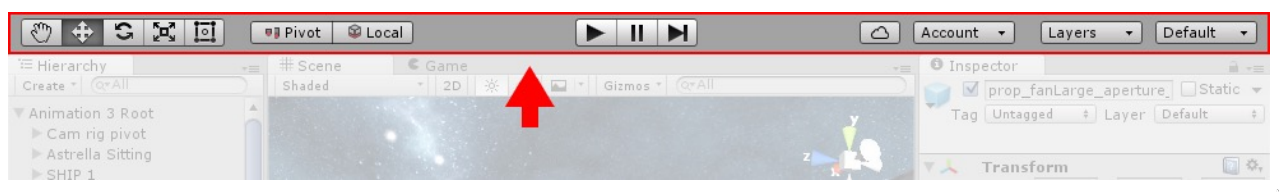
\includegraphics[width=0.9\textwidth]{./images/toolbar.png}
    \caption{The Toolbar}
\end{figure}

\subsubsection{The Game Loop}
At their core, games operate a \textbf{game loop}, although game engines somewhat hide this from you. 
It operates at 60fps (or more), deal with inputs received asynchronously via events (e.g. keyboard or network data) or 
polled for right now, process game objects such as move the physics simulation (if any) forwards or move objects by 
physics simulation or direct control, redraw, wait (maybe) or run at maximum obtainable speed (maybe) but don't block the 
main thread.

\subsubsection{The Unity API}
Luckily, everything is not just drag-n-drop. 
We can write C\# code to make the game work. 
Much of our code will involve the manipulation of the Unity API classes from the \verb|UnityEngine| \& \verb|UnityEngine.UI| 
namespaces. 
Of course, we can also do anything else supported by the core C\#/.NET library such as file handling, networking, collection 
classes, etc.

\subsubsection{Component-Based Architecture}
2\textsuperscript{nd} generation game engines such as Unity3D use \textbf{Component-Based Architecture (CBA)}, which suits
game logic very well. 
It's different to classic OOP as it's based on the \textbf{Composition} rather than \textbf{Inheritance} principle. 
Every \textbf{entity} consists of one or more \textbf{components} which add additional behaviour or functionality. 
The behaviour of an entity can even be changed at runtime by adding or removing components. 
This eliminates the ambiguity problems of inheritance class-hierarchies that are difficult to understand, maintain, \&
extend.
Each component is essentially a separate software object but all attached to some higher-level \verb|GameObject| which 
typically equates to an actual onscreen character, enemy, bullet, effect, vehicle, etc.
\\\\ 
Using composition rather than inheritance can be somewhat of a mantra, and not correct in all cases. 
Code re-use is often (incorrectly) considered to be the main principle of inheritance. 
In fact, designing hierarchical taxonomies of classes is the most appropriate reason to use inheritance. 
Composition is better when you would otherwise get tangles up in the murky world of multiple-inheritance. 
Composition is excellent for code re-use.

\section{Lab Session 1}
Import a model of Mars (and a \verb|texture.jpg| for it). 
Create a simple demo which rotates Mars using the built-in physics engine. 
We could also take direct control of the Mars object and rotate it ourselves, a little bit on each frame, but here we're 
letting the physics engine do the work.
No need to submit anything for this lab session as it's not graded.

\begin{code}
\begin{minted}[texcl, mathescape, linenos, breaklines, frame=single]{csharp}
using System.Collections;
using System.Collections.Generic;
using UnityEngine;

public class GameManagerScript : MonoBehaviour {
    public GameObject marsObject;
    // Use this for initialization
    void Start () {
        Camera.main.transform.position = new Vector3 (0f, 0f, -100f);
        Camera.main.transform.LookAt (marsObject.transform);
        // use the physics engine to rotate Mars
        // before this can run, you need to manually add a rigid body with 0 angular velocity and no gravity in the UI
        marsObject.GetComponent<Rigidbody>().AddTorque (new Vector3(0f,20f,0f));
    }
}
\end{minted}
\caption{Lab 1 Code}
\end{code}

\begin{code}
\begin{minted}[texcl, mathescape, linenos, breaklines, frame=single]{csharp}
public class GameManager : MonoBehaviour {
    // inspector settings
    public GameObject marsObject;
    void Start() {
        marsObject.transform.position = new Vector3(0,0,0);
        Camera.main.transform.position = new Vector3(0,0,100);
        Camera.main.transform.LookAt(marsObject.transform);
    }
    void Update() {
        // programmatically rotate Mars each frame:
        marsObject.transform.Rotate(new Vector3(0,10*Time.deltaTime,0));
    }
}
\end{minted}
\caption{Alternative Lab 1 Code}
\end{code}

\section{Key Concepts \& Classes}
\subsection{\texttt{MonoBehaviour}}
\textbf{\texttt{MonoBehaviour}} is the base class from which Unity C\# scripts normally derive. 
This hooks the class into the Game Loop so that it automatically receives calls to specific methods at specific times. 
It also provides various other useful Unity methods that are called by the game engine in specific situations, including but 
not limited to: 
\begin{multicols}{3}
\begin{itemize}
    \item   \verb|Start()|
    \item   \verb|OnDestroy()|
    \item   \verb|Awake()| 
    \item   \verb|Update()|
    \item   \verb|FixedUpdate()|
    \item   \verb|LateUpdate()|
    \item   \verb|OnDisable()|
    \item   \verb|OnEnabled()|
    \item   \verb|OnBecameInvisible()|
    \item   \verb|OnBecameVisible()|
    \item   \verb|OnCollisionEnter()|
    \item   \verb|OnCollisionExit()|
    \item   \verb|OnCollisionStay()|
    \item   \verb|OnTriggerEnter()|
    \item   \verb|OnTriggerExit()|
    \item   \verb|OnTriggerStay()|
    \item   \verb|OnMouseEnter()|
    \item   \verb|OnMouseExit()|
    \item   \verb|OnMouseDown()|
\end{itemize}
\end{multicols}

In games, it is often useful to be able to execute code at programmer-controlled intervals (perhaps much less often than every 
frame), or at some specified time in the future. 
In Unity \verb|MonoBehaviour|, the methods \verb|Invoke()| \& \verb|StartCoroutine()| relate to this. 
We will elaborate on these later.
\verb|MonoBehaviour| also provides several important data members such as: 
\begin{multicols}{2}
\begin{itemize}
    \item   \verb|enabled| (Boolean).
    \item   \verb|gameObject| (GameObject).
    \item   \verb|transform| (Transform).
    \item   \verb|name| (String) (name of \verb|gameObject|).
\end{itemize}
\end{multicols}

Finally, there are some more methods provided which are useful for manipulating \verb|GameObject|s and their components: 
\begin{multicols}{3}
\begin{itemize}
    \item   \verb|SendMessage()|
    \item   \verb|BroadcastMessage()|
    \item   \verb|SendMessageUpwards()|
    \item   \verb|GetComponent()|
    \item   \verb|GetComponentInChildren()|
    \item   \verb|GetComponentInParent()|
    \item   \verb|GetComponents()|
    \item   \verb|GetComponentsInChildren()|
    \item   \verb|GetComponentsInParent()|
    \item   \verb|GetInstanceID()|
\end{itemize}
\end{multicols}

Recall that \verb|GameObject|s can contain many independent scripts (components), each inheriting from \verb|MonoBehaviour|. 
Each script/component is an instance of a class. 
A \verb|GameObject| is therefore composed of multiple software objects. 
This is called a ``component-based system'' and is often seen as a superior approach to object-oriented class hierarchies -- 
better for code re-use \& isolation of functionality. 
\\\\ 
References:
\begin{itemize}
    \item   \url{https://docs.unity3d.com/ScriptReference/MonoBehaviour.html}
    \item   \url{https://docs.unity3d.com/Manual/ExecutionOrder.html}
\end{itemize}

\subsection{\texttt{GameObject}s in Unity}
\verb|GameObject| is the base class for all entities that exist in a Unity scene. 
As discussed above, each \verb|GameObject| has a collection of components attached, and each component is an independent class 
object inheriting from \verb|MonoBehaviour|. 
The \verb|GameObject| is a special class that \emph{all} entities in the game are derived from and which you won't have to 
attach as a component. 
Some useful data members of \verb|GameObject| include:
\begin{itemize}
    \item   \verb|activeInHierarchy| (Boolean).
    \item   \verb|transform| (Transform). 
    \item   \verb|tag| (Tag type as defined in the editor).
\end{itemize}

Some useful methods of \verb|GameObject| include:
\begin{itemize}
    \item   \verb|AddComponet()|. 
    \item   \verb|SendMessage()| etc. (same as the method in \verb|MonoBehaviour| classes).
    \item   \verb|GetComponent()| etc. (same as the method in \verb|MonoBehaviour| classes).
    \item   \verb|SetActive()|.  
\end{itemize}

Some useful static methods of \verb|GameObject| include:
\begin{itemize}
    \item   \verb|Find()|. 
    \item   \verb|Destroy()|. 
    \item   \verb|Instantiate()|. 
\end{itemize}

\subsubsection{Getting References to \texttt{GameObject}s at Runtime}
For a specific \verb|GameObject|:
\begin{itemize}
    \item   Have it referenced as a public member of the script that needs it, and associated at design-time in the Inspector.
            (This is what we did in the first lab for the Mars object, a reference to which was needed by the
            \verb|GameManager| class).
    \item   Use \verb|GameObject.Find("<name>")| to find it by name. This is somewhat inefficient, so don't do this every frame. 
    \item   Use \verb|GameObject.FindGameObjectsWithTag("<tag>")| to find all game objects with a specified tag. This returns an array
            of \verb|GameObject|s.
\end{itemize}

\subsubsection{Prefabs}
When you have created a \verb|GameObject| in the hierarchy (at design time), added components to it, and set their various 
public values, you can drag the \verb|GameObject| into the Assets Window to make a \textbf{prefab}, essentially a template of 
that exact object with its settings. 
\\\\
This approach means that you can make \verb|MonoBehaviour| scripts for monsters, guns, etc. and then make a separate prefab 
with different settings for each actual type of monster or gun you need in your game.
Prefabs are therefore useful for creating \& editing your game's data. 
 
\subsubsection{Runtime Instantiation \& Destruction of \texttt{GameObject}s}
So far, we have created all of the \verb|GameObject|s that we need in the hierarchy at design-time (i.e., before starting the
game).
Often, we need to instantiate \& destroy some or all of our game objects at runtime, e.g. bullets, enemies, explosions, etc. 
Assuming that we have a \textbf{prefab} in our Assets, and that it is located in a directory called \verb|Resources| we can 
do the following.
Here, \verb|prefabName| is the name of our asset prefab (as a String):
\begin{minted}[texcl, mathescape, linenos, breaklines, frame=single]{csharp}
GameObject go = Instantiate(Resources.Load(prefabName));

// later on, assuming we  still have a reference to the object:
GameObject.Destroy(go);
// or 
GameObject.DestroyImmediate(go);
\end{minted}

Alternatively, you can instantiate an object by supplying an existing instantiated object as a template. 
E.g., in Lab 1 our \verb|GameManagerScript| class had a \verb|GameObject| member called \verb|marsObject|, which is 
instantiated in the Inspector at design time, so you could use this to make another Mars:
\begin{minted}[texcl, mathescape, linenos, breaklines, frame=single]{csharp}
GameObject otherMarsObject = Instantiate(marsObject);
\end{minted}

Another alternative, perhaps the easiest of all, is to have a public reference to a \verb|GameObject| and associate this
with a prefab in the assets by dragging in the Inspector. 
Then you can use \verb|Instantiate()| on that to instantiate a copy of the prefab into the scene at runtime.

\subsubsection{Cameras}
In computer graphics, \textbf{Cameras} are software objects that define a viewpoint in terms of position, orientation, 
field-of-view/zoom, etc. within the ``virtual world''.
Mathematical projections are used to calculate how the 3D world should be displayed on the 2D camera surface. 
In Unity, Cameras are \verb|GameObject|s which have a \verb|Camera| component. 
Since they're \verb|GameObject|s, you can add other components, manipulate their \verb|Transform|, etc. just like any other 
\verb|GameObject|. 
The \verb|Transform| component provides methods that are very useful to Cameras (as well as other non-Camera objects) such as 
\verb|LookAt()|. 
\\\\ 
\verb|Camera.main| is a static reference to the ``main'' Camera whose view is being displayed to the screen. 
This Camera should have the tag \verb|MainCamera|. 
Other Cameras can be used at the same time, e.g. to render to texture (e.g. mirrors, top-down minimaps) or to render to parts
of the screen (e.g., split-screen multiplayer).
You might also have multiple cameras in a scene and switch the active one during the game.
\\\\ 
The \verb|Camera| class provides methods for converting co-ordinates between Screen-space, Viewport-space, \& World-space 
(more on these later).
\begin{itemize}
    \item   \verb|CalculateFrustumCorners()|:  Given viewport coordinates, calculates the view space vectors pointing to the
            four frustum corners at the specified camera depth.
    \item   \verb|ScreenPointToRay()|:  Returns a ray going from camera through a screen point.
    \item   \verb|ScreenToViewportPoint()|:  Transforms position from screen space into viewport space.
    \item   \verb|ScreenToWorldPoint()|:  Transforms position from screen space into world space.
    \item   \verb|ViewportPointToRay()|: Returns a ray going from camera through a viewport point. 
    \item   \verb|ViewportToScreenPointTransforms()|: position from viewport space into screen space. 
    \item   \verb|ViewportToWorldPointTransforms()|: position from viewport space into world space. 
    \item   \verb|WorldToScreenPointTransforms()|: position from world space into screen space. 
    \item   \verb|WorldToViewportPointTransforms()|: position from world space into viewport space.
\end{itemize}
References:
\begin{itemize}
    \item   \url{https://docs.unity3d.com/ScriptReference/Camera.html}
    \item   \url{https://docs.unity3d.com/Manual/class-Camera.html}
\end{itemize}

\subsubsection{Transforms}
A \textbf{Transform} defines the position, orientation, \& scale of an object. 
Child objects have their own Transforms which are interpreted as a nested co-ordinate system, i.e. a modification of the
parent's.
This is a very powerful concept and is fundamental to the concept of a SceneGraph/hierarchy.
In Unity, the \verb|Transform| class has the following key members: 
\begin{itemize}
    \item   \verb|position| (Vector3)
    \item   \verb|localPosition| (Vector3)
    \item   \verb|rotation| (Quaternion)
    \item   \verb|localRotation| (Quaternion)
    \item   \verb|lossyScale| (Vector3)
    \item   \verb|localScale| (Vector3)
    \item   \verb|parent| (Transform)
    \item   \verb|right|: positive direction on the local x axis (Vector3, normalised).
    \item   \verb|up|: positive direction on the local y axis (Vector3, normalised).
    \item   \verb|forward|: positive direction on the local z axis (Vector3, normalised).
    \item   \verb|gameObject| (GameObject)
\end{itemize}

Methods of the \verb|Transform| class include:
\begin{itemize}
    \item   \verb|Rotate()|: Uses ``Euler angles'' ($x$, $y$, $z$) all in degrees.
    \item   \verb|Translate()|
    \item   \verb|TransformPoint()|: Transforms position from local space to world space.
    \item   \verb|InverseTransformPoint()|: Transforms position from world space to local space.
    \item   \verb|LookAt()|: (Vector3 point) turns so that the forward direction (i.e., positive $z$ axis) faces the specified 
            position.
    \item   \verb|RotateAround()|: (Vector3 point, Vector3 axis, float degrees).
    \item   \verb|SetParent()|
\end{itemize}

Reference: \url{https://docs.unity3d.com/ScriptReference/Transform.html}

\subsubsection{Skyboxes}
\textbf{Skyboxes} are rendered around the whole scene in the background in order to give the impression of complex scenery at 
the horizon. 
To implement a Skybox, create a Skybox Material in your Assets. 
Then, add it to the scene by using the Window {\rightarrow} Rendering {\rightarrow} Lighting menu item and specifying your Skybox 
material as the Skybox on the Scene tab.
\\\\
Reference: \url{https://docs.unity3d.com/Manual/class-Skybox.html}

\subsubsection{Keyboard Input}
We will revisit more details about Keyboard/Mouse/Joystick/Touchscreen input later, but for now we will just say that 
\verb|Input.GetKey()| returns true as long as a key is held down. 
E.g., this could be written in an \verb|Update()| method: 
\begin{minted}[texcl, mathescape, linenos, breaklines, frame=single]{csharp}
if (Input.GetKey(KeyCode.LeftArrow)) {
    RotateCameraAroundMarsSomehow();
}
\end{minted}

References:
\begin{itemize}
    \item   \url{https://docs.unity3d.com/ScriptReference/Input.html}
    \item   \url{https://docs.unity3d.com/ScriptReference/Input.GetKey.html}
\end{itemize}

\subsubsection{Static Member Variables}
By declaring a member variable \textbf{\texttt{static}}, you're creating a single copy of the variable which is owned by the
class rather than by any specific instance object. 
Each instance does not have its own unique copy, they share one.
A common use case for static member variables is if you want to retain a collection of all instances of the class for quick 
recall.

\subsubsection{Static Member Functions}
By declaring a method \textbf{\texttt{static}}, you're creating a method that is called on the class itself, not an instance of 
it. 
This is very useful since you don not need to have a reference to an instantiated object from the class in order to call it. 
For obvious reasons, a static method only has access to static member variables of the class, while a non-static method 
(which is called on an actual instantiated object) has in addition, access to its own copies of non-static member variables.

\subsubsection{The Singleton Pattern}
A common design approach in Unity is to create single-instance \textbf{singleton} classes for various ``management'' roles,
e.g. \verb|GameManager|, \verb|GUIManager|, \verb|AudioManager|, \verb|SaveGameManager|, etc.
The typical approach is to create a \verb|GameObject| in the hierarchy which holds the one-and-only instance of these 
components that will exist at run-time.
One habit is to attach these to the Main Camera.
Using statics can make the methods of these management singletons very easy \& clean to access, e.g. consider the ``instance'' 
static member variable used here; it gives direct access to data attached to the instantiated singleton object, from anywhere 
in the game, via \verb|GameManager.instance|
\begin{minted}[texcl, mathescape, linenos, breaklines, frame=single]{csharp}
public class GameManager : MonoBehaviour {
    public static GameManager instance;

    void Start () {
        instance = this;
    }
}
\end{minted}

\subsection{Lab 2: Fear \& Dread}
In our first lab, we attached a \verb|Rigidbody| to the Mars object, applied angular velocity to it using \verb|AddTorque|, 
and let the game engine control the movement of it. 
The other way of moving game objectsis to directly manipulate their \verb|Transform| using code (this was our approach in
second year Java).
In Lab 2, we'll be making Mars' two moons (Phobos \& Deimos) orbit around it through direct manipulations of their Transforms. 
Your code for doing this would typically be written in the \verb|Update()| method of some script (it could either be a 
script attached to the \verb|GameObject| itself, or perhaps a script attached to a singleton ``manager'' object). 
It is important to consider the fact that \verb|Update()| is probably not happening at fixed time intervals. 
You can multiply all movement code by \verb|Time.deltaTime|.

\section{Co-ordinate Systems}    
The most important co-ordinate system distinction in Unity is between the \textbf{Global} (or World) co-ordinate system 
and the \textbf{Local} co-ordinate system of each \verb|GameObject|.
Hence, to rotate the camera round the $y$-axis \emph{as perceived by the camera} (i.e., the $y$-axis of its Local Co-ordinate
system) we can use:
\begin{minted}[texcl, mathescape, linenos, breaklines, frame=single]{csharp}
camera.transform.RotateAround(Vector3.zero, camera.transform.up, 50f * Time.deltaTime);
\end{minted}

Or, to rotate it around the Global $y$-axis:
\begin{minted}[texcl, mathescape, linenos, breaklines, frame=single]{csharp}
camera.transform.RotateAroudn(Vector3.zero, Vector3.up, 50f * Time.deltaTime);
\end{minted}

The first \verb|Vector3| argument defines the world point around which to rotate.
\\\\ 
Some methods of the \verb|Transform| class for translating from the local space of a transform to global space and 
vice-versa include:
\begin{minted}[texcl, mathescape, linenos, breaklines, frame=single]{csharp}
// local space to global
public Vector3 TransformPoint(Vector3 position);
public Vector3 TransformDirection(Vector3 direction);
public Vector3 TransformVector(Vector3 vector);
// global to local
public Vector3 InverseTransformPoint(Vector3 position);
public Vector3 InverseTransformDirection(Vector3 direction);
public Vector3 InverseTransformVector(Vector3 vector);
\end{minted}

\subsection{Examples}
To find the world-coordinate of a point which is 10 units ``in front of'' a spaceship (in terms of its 
own direction facing, and assuming this code is located inside a script attached to the spaceship):
\begin{minted}[texcl, mathescape, linenos, breaklines, frame=single]{csharp}
Vector3 pt = transform.TransformPoint(new Vector3(0f, 0f, 10f));
// another way of doing the same would be: 
Vector3 pt = transform.position + 10f * transform.forward;
\end{minted}

To accelerate a spaceship forwards (assuming it has a \verb|Rigidbody| and we're using physics, and we're doing this in a 
\verb|FixedUpdate()| method on one of its scripts):
\begin{minted}[texcl, mathescape, linenos, breaklines, frame=single]{csharp}
Rigidbody rigid = GetComponent<Rigidbody>();
rigid.AddForce(transform.forward * 200f * Time.fixedDeltaTime);
\end{minted}

To get the direction \& distance between two \verb|GameObject|s:
\begin{minted}[texcl, mathescape, linenos, breaklines, frame=single]{csharp}
GameObject go1, go2; // it's assumed that these are not nulls!

Vector3 difference, direction; 
difference = go2.transform.position - go1.transform.position;
direction = difference.normalized;
float distance = difference.magnitude;
\end{minted}

Iterating nested objects using \verb|foreach (Transoform t in Transform)|:
\begin{minted}[texcl, mathescape, linenos, breaklines, frame=single]{csharp}
public class Area : MonoBehaviour {
    // inspector settings 
    public Transform innerWallsGroup;
    public Vector3 wallsPos;

    private List<GameObject> innerWalls = new List<GameObject>();
    private bool[] wallIsRaised = null;

    void Start() {
        foreach (Transform t in innerWallsGroup) {
            innerWalls.Add(t.gameObject);
        }

        wallIsRaised = new bool[innerWalls.Count];

        for (int i = 0; i < innerWalls.Coutn; i++) {
            innerWalls[i].transform.position = wallsPos;
            innerWalls[i].SetActive(false);
            wallIsRaised[i] = false;
        }
    }
}
\end{minted}

\subsection{Screen Space, Viewport Space, \& World Space}
Reference: \url{https://docs.unity3d.com/ScriptReference/Camera.html}
\\\\
The \verb|Camera| class provides methods for translating between three different ``spaces'', i.e. different ways of 
mapping the positions of things. 
\\\\
Each of these is stored as a \verb|Vector3| (which is a \verb|struct|).
A \textbf{screen space} point is defined in pixels. 
The bottom-left of the screen is $(0,0)$; the right-top is $(\texttt{Camera.pixelWidth}, \texttt{Camera.pixelHeight})$ . 
If you're using a \verb|Vector3| rather than a \verb|Vector2|, then the $z$ position is in \textbf{world units} in front 
of the Camera, rather than in screen pixels.
See also the \verb|Screen| class: \url{https://docs.unity3d.com/ScriptReference/Screen.html}
\\\\ 
A \textbf{viewport space} point is normalised and relative to the Camera. 
The bottom-left of the Camera is $(0,0)$; the top-right is $(1,1)$.
Again, the $z$ position (if any) is in world units in front of the Camera.
E.g., this is appropriate for positioning GUI elements independent of actual pixel resolution of the screen.
\\\\ 
A \textbf{world space} is defined in global co-ordinates (for example, \verb|transform.position|. 
E.g., this is appropriate for \verb|GameObject|s in the game world. 
\verb|GameObject|s which are nested in the Hierarchy have both \verb|transform.position| \&
\verb|transform.localPosition|; \verb|transform.rotation| \& \verb|transform.localRotation|, etc.

\subsubsection{Typical Space-Translation Operations}
Find where the mouse is in world co-ordinates to see if a \verb|GameObject| is under the mouse:
\begin{minted}[texcl, mathescape, linenos, breaklines, frame=single]{csharp}
// note that Input.mousePosition gives a Vector4 where the $z$ component is 0 
// the screen is 2D of course; the $z$ component of the Vector3 supplied to ScreenToWorldPoint is a world-coordinate distance into the world.
Vector3 mousePosInWorld = Camera.main.ScreenToWorldPoint(Input.mousePosition);
\end{minted}

Find a \verb|GameObject| in screen-pixel coordinates to position a GUI item such as a healthbar above it:
\begin{minted}[texcl, mathescape, linenos, breaklines, frame=single]{csharp}
GameObject targ; // assumed not to be null
Vector3 screenPos = Camera.main.WorldToScreenPoint(targ.transform.position);
\end{minted}

\begin{code}
\begin{minted}[texcl, mathescape, linenos, breaklines, frame=single]{csharp}
// Here, we find the 3D position that's just above the enemy's head, and convert this to a vieweort position when viewed through the player's camera.
// Finally, this viewport position is converted to a pixel position as required by the GUI sprite.
public class MonsterManager : MonoBehaviour {
    void Update () {
        if (GameManager.gameState==GameStates.Playing) {
            if (numMonstersAlive==1) {
                // put the final enemy indicator (GUI object) above the final monster
                GameObject go = GUIManager.instance.finalEnemyIndicator;
                Monster m = allActiveMonsters[0];
                Bounds b = m.mycollider.bounds;
                Vector3 pos = new Vector3(b.center.x, b.max.y + 1f, b.center.z);
                Vector3 viewPos = Player.myPlayer.fpsCamera.WorldToViewportPoint(pos);
                if (viewPos.x<0f || viewPos.x>1f || viewPos.y<0f || viewPos.y>1f || viewPos.z<0f)
                    go.SetActive(false);
                else { 
                    go.SetActive(true);
                    go.transform.position = new Vector2(viewPos.x*Screen.width, viewPos.y*Screen.height);
                }
            }
        }
    }
}
\end{minted}
\caption{The ``Final Enemy Indicator'' in DemonPit}
\end{code}

\section{Object Interactions with Colliders \& Triggers}
Objects which have \verb|Collider|s \& \verb|Rigidbody|s will physically respond to impacts (i.e., they'll bounce off each
other). 
Objects which have Triggers but not Colliders will \textbf{not} physically interact. 
\\\\ 
Related to the physics engine are two sets of \verb|MonoBheaviour| methods which are called automatically when objects 
with Colliders or Triggers interact: 
\begin{minted}[texcl, mathescape, linenos, breaklines, frame=single]{csharp}
// these happen for Collider-to-Collider collisions
OnCollisionEnter(Collision coll);
OnCollisionExit(Collision coll);
OnCollisionStay(Collision coll);

// these happen for Trigger-to-Trigger collisions
OnTriggerEnter(Collider coll);
OnTriggerExit(Collider coll);
OnTriggerStay(Collider coll);
\end{minted}

The \verb|Collision| argument provides information on the game object that has collided with us, as well as additional 
information about the collision itself (e.g., the speed of impact). 
The \verb|Collider| argument is simply a reference to the Trigger component that interact with ours. 
\verb|OnCollision| refers to an actual physics interaction between two Colliders (e.g. \verb|BoxCollider| or
\verb|SphereCollider| components). 
\verb|OnTrigger| is the same thing except here the Collider has its Trigger flag set to \verb|true|. 
Triggers enable game-logic interaction when you don't want physical collision responses.
\\\\
Reference: \url{https://docs.unity3d.com/ScriptReference/Collider.OnCollisionEnter.html}

\subsection{Lab 3: Asteroid Assault on Mars \& its Moons}
This lab builds on the work from the last two weeks; we already have Mars rotating, with Phobos \& Deimos orbiting around 
it, and keyboard control of the camera. 
This week, we will be instantiating asteroids at runtime, and setting them moving (using physics). 
Asteroid which collide with anything will be destroyed, as will be asteroids which pass offscreen.

\subsection{Triggers (Sensors)}
\textbf{Triggers} are invisible components that are activated (triggered) when a character or other object passes inside 
them. 
They are a very common \& useful mechanism in games. 
In Unity, Trigger is made by using a Collider with its Trigger property checked. 

\subsection{Coroutines}
\textbf{Coroutines} are special functions that can pause their execution.
They're very useful for delayed execution, making things happen in steps (with a defined delay between each step), or for 
waiting for something else to complete before executing.
Coroutines are a very useful feature provided by the \verb|MonoBehaviour| class.
Their usefulness is because the code related to something occurring in the game is kept all in one place, even if that 
something takes a long time to occur, or occurs in stages.
Coroutines are not threads, as they run in the same thread as the main Unity process, but they are much simpler to use than 
threads. 
In any case, most of the Unity SDK is not thread-safe.
Coroutines are started with a call to \verb|StartCoroutine()|, and they must have the \verb|IEnumerator| return type.
Technically, the way that these work is that Unity maintains a list of active Coroutines and on each game loop wakes up 
any that are now due to wake up.
\\\\ 
When the coroutine is activated, it well execute until the next \verb|yield| statement and then pause until it is 
resumed.
Various values can be supplied with the \verb|yield| statement, e.g. \verb|yield return null| simply waits until the next
frame.
\begin{minted}[texcl, mathescape, linenos, breaklines, frame=single]{csharp}
private void Start() {
    Debug.Log("Start method");
    StartCoroutine(TestCoroutine());
    Debug.Log("Start method ends");
}

// this coroutine has a loop that runs as along as the calling object is active
private IEnumerator TestCoroutine() {
    Debug.Log("TestCoroutine");
    while(true)
    {
        Debug.Log("Here");
        yield return null;
        Debug.Log("There");
    }
}

private void Update() {
    Debug.Log("Update");
}

// Output should be:
/*
Start method
TestCoroutine
Here
Start method ends
Update
There
Here
Update
There
Here
*/
\end{minted}

Some of the most useful Coroutine \verb|yield| values include:
\begin{itemize}
    \item   \verb|yield return null;| -- the coroutine is continued the next time that it is eligible, normally on the
            next frame.
    \item   \verb|yield return new WaitForSeconds(3f);| -- causes the coroutine to pause for a specified time period (three
            seconds in this example). Be aware of the garbage implications of this.
    \item   \verb|yield return StartCoroutine(OtherCoroutine());| -- waits until the other coroutine has run to completion
            before the yielder is resumed.
    \item   \verb|yield break;| -- stops the coroutine and exits (i.e., this is the equivalent of a \verb|return| statement
            in a normal method).
\end{itemize}

Be aware of changes during the \verb|yield| time. 
You always have to be careful with asynchronous programming: something important may have changed during the ``down time''
of a coroutine.
\\\\
Reference: \url{https://unitygem.wordpress.com/coroutines/}

\subsubsection{\texttt{Invoke} \& \texttt{InvokeRepeating}}
\verb|Invoke| \& \verb|InvokeRepeating| provide a simpler way of running a complete method some time in the future, either 
as a one-off or a repeating call.
\begin{minted}[texcl, mathescape, linenos, breaklines, frame=single]{csharp}
public class ExampleScript : MonoBehaviour
{
    // Launches a projectile after 2 seconds

    Rigidbody projectile;

    void Start() {
        Invoke("LaunchProjectile", 2f);
    }

    void LaunchProjectile()
    {
        Rigidbody instance = Instantiate(projectile);
        instance.velocity = Random.insideUnitSphere * 5f;
    }
}
\end{minted}

To invoke repeatedly:
\begin{minted}[texcl, mathescape, linenos, breaklines, frame=single]{csharp}
InvokeRepeating("LaunchProjectile", 2.0f, 0.3f);
\end{minted}

\subsection{Layers}
\textbf{Layers} allow you to group game objects into categories.
They are can be found at Edit {\rightarrow} Project Settings {\rightarrow} Tags and Layers.
You can then decide which layers interact with each other in the physics simulation.
You can also use an object's Layer to decide what happens when it collides with another object.
You can also apply raycasts (see later) on specific objects only, e.g. to determine whether a monster can see a player, 
you would cast a ray between the position of the monster's head and the player's head, but only let the raycast consider
walls/floors, i.e. it would ignore any creatures in the way.
\\\\ 
Don't confuse Layers with Sorting Layers: the latter is for deciding the draw order of Sprites.
\\\\
Reference: \url{https://docs.unity3d.com/560/Documentation/Manual/Layers.html}

\section{Physics}
\subsection{Rigidbody}
References:
\begin{itemize}
    \item   \url{https://docs.unity3d.com/Manual/RigidbodiesOverview.html}
    \item   \url{https://docs.unity3d.com/ScriptReference/Rigidbody.html}
\end{itemize}

A \verb|Rigidbody| is the main component that enables phyiscal behaviour for a \verb|GameObject|;
it puts the \verb|GameObject| under the control of the physics engine.
The object will respond to gravity if it has a \verb|Rigidbody| component attached, (provided that the \verb|useGravity| 
field is not set to \verb|false|.
If one or more Collider components are added, the \verb|GameObject| is affected by incoming collisions (from other Colliders)
according to its shape, mass, momentum, linear, \& angular velocities, as well as Physics Materials which defined 
bounciness \& friction.
\\\\
Since a \verb|Rigidbody| component takes over the movement of the \verb|GameObject| that it's attached to, you normally
shouldn't try to move it from a script by changing the Transform properties such as position \& rotation; instead you 
should apply forces to push the \verb|GameObject| and let the physics engine calculate the results.
When a \verb|Rigidbody| is moving slower than a defined minimum linear or rotational speed, the physics engine assumes
that it has come to a halt.
When this happens, the \verb|GameObject| does not move again until it receives a collision or force, and so it is set to 
``\textbf{sleeping}'' mode.
This optimisation means that no processor time is spent updating the \verb|Rigidbody| until the next time that is 
``awoken'', i.e. set in motion again.
Sleeping can also be useful as it removes small ``jitters'' that may happen due to inaccuracies in the physics simulation.
In your scripts which apply physics forces to Rigidbodies, use the \verb|FixedUpdate()| method rather than the
\verb|Update()| method, since \verb|FixedUpdate()| is synced with the physics simulation updates.
\\\\ 
\verb|Rigidbody| properties:
\begin{itemize}
    \item   \mintinline{csharp}{public float drag}
    \item   \mintinline{csharp}{public float angularDrag}
    \item   \mintinline{csharp}{public float mass}
    \item   \mintinline{csharp}{public Vector3 velocity}
    \item   \mintinline{csharp}{public Vector3 angularVelocity}
    \item   \mintinline{csharp}{public Vector3 centerOfMass} (offset from Transform centre).
\end{itemize}

\verb|Rigidbody| methods
\begin{itemize}
    \item   \mintinline{csharp}{public void AddForce(Vector3 force)} (\verb|force| is a vector in world co-ordinates
            applied through the centre of mass of the \verb|Rigidbody|.
    \item   \mintinline{csharp}{public void AddRelativeForce(Vector3 force)} (\verb|force| is a vector in local
            co-ordinates).
    \item   \mintinline{csharp}{public void AddForceAtPosition(Vector3 force, Vector3 position)}

\end{itemize}

\subsection{Colliders}
Reference: \url{https://docs.unity3d.com/Manual/CollidersOverview.html}
\\\\
\textbf{Collider} components define the shape of an object for the purposes of physical collisions. 
Colliders are invisible at runtime, and do not need to be the exact same shape as the object's mesh; a rough 
approximation is of the shape is often more efficient, and is indistinguishable in gameplay.
The simplest (\& least processor-intensive) colliders are the \textbf{primitive} collider types, which all
inherit from the superclass \verb|Collider|. 
In 3D, these are the \verb|BoxCollider|, \verb|SphereCollider|, \& \verb|CapsuleCollider|.
In 2D, these are \verb|BoxCollider2D| \& \verb|CircleCollider2D|. 
Any number of these can be added to a single object to create composite colliders to reasonably approximate a 3D
model.
\\\\
If you need more accuracy (at increased processor cost), use \textbf{\texttt{MeshCollider}} which accurately 
matches the 3D graphical model (the polygonal mesh). 
A \verb|MeshCollider| will be unable to collide with another \verb|MeshCollider| unless you mark it as
\verb|Convex| in the inspector.
This will generate the collider shape as a ``convex hull'' which is like the original mesh with concavities 
filled in.
The general rule is to use mesh colliders for static scene geometry (walls, ground, etc.) and to approximate the 
shape of moving objects using composite primitive colliders.
\begin{figure}[H]
    \centering
    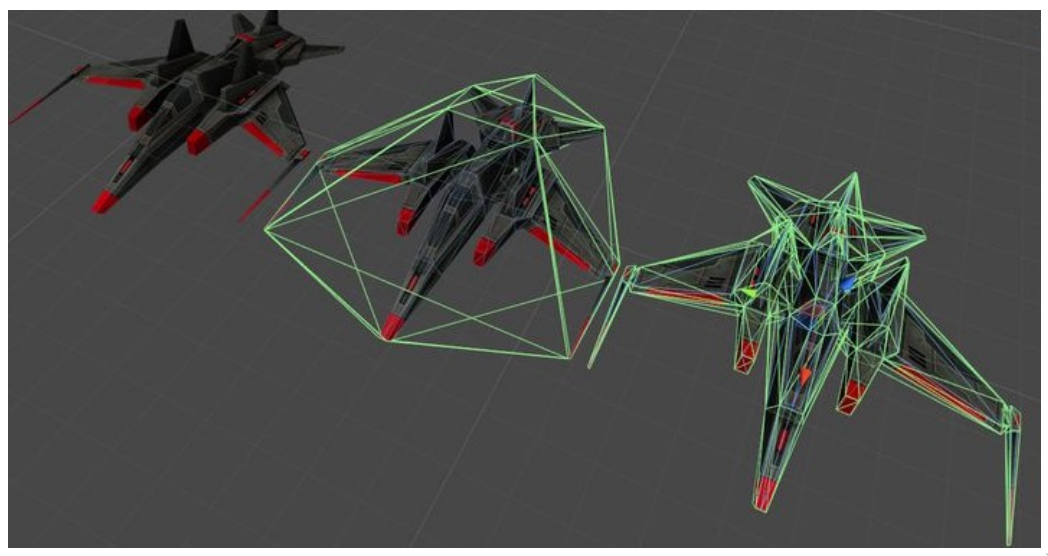
\includegraphics[width=0.7\textwidth]{./images/MeshCollider.png}
    \caption{\texttt{MeshCollider}: Convex Hull vs Non-Convex}
\end{figure}

\begin{figure}[H]
    \centering
    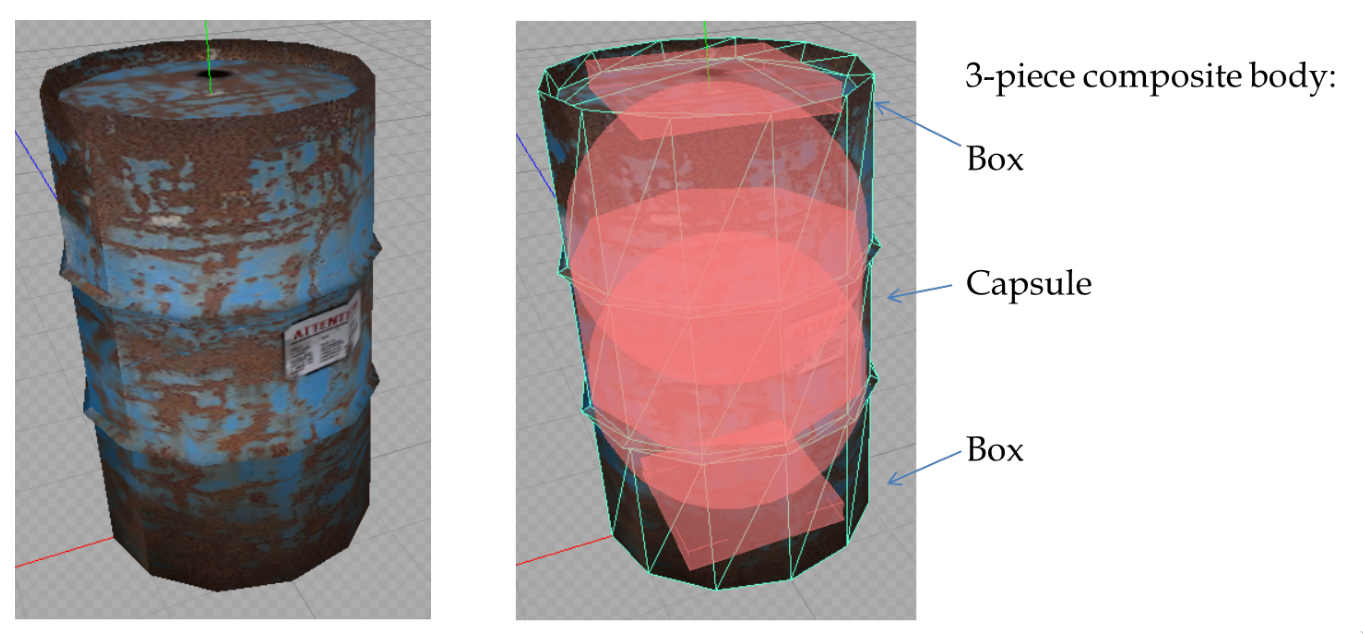
\includegraphics[width=0.7\textwidth]{./images/CompositeCollider.png}
    \caption{Composite Collider}
\end{figure}

\subsubsection{Collisions}
Reference: \url{https://docs.unity3d.com/ScriptReference/Collision.html}
\\\\
Any object with a Collider receives messages from the physics engine when it collides with other Colliders.
Any script on the object may choose to respond by implementing the following methods:
\begin{itemize}
    \item   \mintinline{csharp}{void OnCollisionEnter(Collision collision)} (the \verb|Collision| object contains
            information about contact points, impact velocity, etc.)
    \item   \mintinline{csharp}{void OnCollisionExit(Collision collision)}
    \item   \mintinline{csharp}{void OnCollisionStay(Collision collision)}
\end{itemize}

The \verb|OnCollision| methods receive objects of type \verb|Collision|, which contain useful information such as:
\begin{itemize}
    \item   \verb|collider|: The \verb|Collider| object that was hit.
    \item   \verb|contacts|: The contact point(s) generated by the physics engine as an array of
            \verb|ContactPoint| structs.
    \item   \verb|gameObject|: The \verb|GameObject| whose collider was collided with.
    \item   \verb|relativeVelocity|: The relative linear velocity of the two colliding objects as a \verb|Vector3|.
    \item   \verb|rigidbody|: The \verb|Rigidbody| that was hit; this is \verb|null| if the object had a collider
            but no \verb|Rigidbody|.
\end{itemize}

\subsubsection{\texttt{ContactPoint} Struct}
Reference: \url{https://docs.unity3d.com/ScriptReference/ContactPoint.html}
\\\\
\verb|Collision| objects contain arrays of \verb|ContactPoint| structs in their \verb|.contacts| member variable.
The member data of the \verb|ContactPoint| struct is as follows:
\begin{itemize}
    \item   \verb|point|: The point of contact in \verb|Vector3| world co-ordinates.
    \item   \verb|normal|: The surface normal at the contact point in \verb|Vector3|.
    \item   \verb|otherCollider|: The other \verb|Collider| in contact at the point.
    \item   \verb|thisCollider|: The first collider in contact at the point (useful if a \verb|GameObject| has 
            more than one \verb|Collider| and we need to know which one).
\end{itemize}

These fields allow us to operate on the object that we hit and to create accurate special effects etc. at the 
point of contact, rotated according to the surface normal at that point.

\subsubsection{\texttt{PhysicMaterial}}
When Colliders interact, their surfaces need to simulate the properties of the material that they are supposed to
represent.
For example, a sheet of ice will be slippery while a rubber ball will offer a lot of friction and be very bouncy.
Although the shape of colliders is not deformed during Collisions (hence the term ``rigid body physics''), their
friction \& bounce can be configured using \verb|PhysicMaterial|s.














\end{document}
